\documentclass[aspectratio=169,11pt]{beamer}
\usetheme{Madrid}
\usecolortheme{seahorse}
\usepackage[T1]{fontenc}
\usepackage{lmodern}
\usepackage{booktabs,graphicx,amsmath,tikz,xcolor,array}
\usetikzlibrary{shapes,arrows.meta,positioning}
\definecolor{good}{RGB}{30,130,76}
\definecolor{bad}{RGB}{192,57,43}
\setbeamertemplate{navigation symbols}{}
\title[AnomalyGFM extensions]{Extending AnomalyGFM: What Helps, What Doesn't, and Why}
\subtitle{Zero/few-shot graph anomaly detection with a graph foundation model}
\author{Term project team}
\date{\today}

\begin{document}
\begin{frame}\titlepage\end{frame}

\begin{frame}{Outline}
\tableofcontents
\end{frame}

\section{The paper}
\begin{frame}{AnomalyGFM (KDD'25): the problem}
\begin{columns}[T]
\column{0.5\textwidth}
\begin{itemize}
\item \textbf{Graph anomaly detection (GAD):} flag nodes unlike the majority (fraud accounts, fake reviews).
\item Classical GAD trains and tests on \emph{one} graph $\Rightarrow$ no transfer to unseen graphs.
\item Generic graph foundation models fail on GAD: anomalies are rare, irregular, heterogeneous.
\item \textbf{Goal:} one model, pre-trained once, that detects anomalies in a new graph with \alert{zero labels} (zero-shot) or a few labelled normal nodes (few-shot).
\end{itemize}
\column{0.5\textwidth}
\includegraphics[width=\linewidth]{../framework.png}
\end{columns}
\end{frame}

\begin{frame}{How AnomalyGFM scores a node}
\begin{enumerate}
\item Project every graph to $d'=8$ dims with a fixed \textbf{SVD}; encode with a 2-layer \textbf{GCN}.
\item \textbf{Residual:} $r_v = h_v - \sum_{u\in\mathcal N(v)} w_{vu}h_u$ \quad(small for normal nodes, large for anomalies, in \emph{any} graph).
\item Two learnable \textbf{prototypes} $p_n,\,p_a$ (noise $\to$ linear+ReLU), trained with labelled anomalies on one graph (Facebook, 30\% labelled).
\item \textbf{Zero-shot score:} $\;s_v=\exp\!\big(\cos(r_v,\,p_a)\big)$ --- no tuning on the target.
\item \textbf{Few-shot:} tune a small prompt with $k$ labelled normal nodes.
\end{enumerate}
\vspace{4pt}
\begin{block}{Our question}
Which parts of this pipeline are weak, and can we improve accuracy, label-efficiency or parameter-efficiency?
\end{block}
\end{frame}

\section{Setup}
\begin{frame}{Experimental setup (real data only)}
\begin{columns}[T]
\column{0.55\textwidth}
\begin{itemize}
\item \textbf{Train:} Facebook (1,081 nodes, 2.3\% anomalies)
\item \textbf{Test (zero-shot):} Amazon (11,944), Amazon-UPU (10,224), Reddit (10,984)
\item \textbf{5 seeds}, mean$\pm$std; AUROC and AUPRC
\item Same node set for every row (target minus the 100 tuned normal nodes)
\item \textbf{Also:} in-domain AUROC on held-out Facebook nodes (is the module learning at all?)
\end{itemize}
\column{0.45\textwidth}
\begin{block}{Infrastructure}
\small RTX 4500 Ada (24 GB); code local, runs on server via \texttt{sync.sh}; sparse GPU inference; harness verified: sparse = dense results (Amazon 0.9026, Reddit 0.5952).
\end{block}
\begin{alertblock}{Raw features}
\small Shared files hold only 8-dim SVD; we fetched raw features (labels verified identical) for the hypernetwork.
\end{alertblock}
\end{columns}
\end{frame}

\section{Benchmark: scoring and features}
\begin{frame}{Weaknesses we looked for}
\begin{columns}[T]
\column{0.5\textwidth}
\begin{itemize}
\item[P1] Inference prompts are random noise
\item[P2] Score uses direction only (ignores residual size)
\item[P3] One abnormal prototype for heterogeneous anomalies
\item[P4] Residual = plain neighbour mean (camouflage)
\item[P5] No test-time adaptation (Reddit $\approx0.57$)
\item[P6] Hand-tuned fusion weight in released code
\end{itemize}
\column{0.5\textwidth}
\textbf{Exp I} -- is a better \emph{scoring function} available? (10 scorers)\\[4pt]
\textbf{Exp H} -- is a better \emph{feature alignment} available? (dim $\times$ normalisation, 16 configs)\\[4pt]
9 target graphs $\times$ 5 seeds $\times$ 80 trained models $=$ 7,200 result rows.
\end{columns}
\end{frame}

\begin{frame}{Exp I: no scorer beats the paper's abnormal score}
\centering\small
\begin{tabular}{lcc}
\toprule
Scorer & Mean AUROC (9 graphs) & vs paper \\ \midrule
\textbf{abnormal-prototype cosine (paper)} & \textbf{0.603} & -- \\
rank-fuse(abnormal, residual norm) & 0.592 & $-0.011$ (n.s.) \\
Mahalanobis of residual & 0.558 & $-0.045$ ($p{=}0.16$) \\
residual magnitude only & 0.536 & $-0.067$ \\
Euclidean to prototypes & 0.498 & $-0.105$ \\
\textcolor{bad}{paper's \emph{normal} score / code's fusion} & \textcolor{bad}{0.398} & \textcolor{bad}{$-0.205$ (inverted)} \\
\bottomrule
\end{tabular}
\vspace{6pt}
\begin{itemize}
\item The \emph{normal}-prototype score is worse than chance on 7 of 9 graphs; sign-flipped it ties the abnormal score $\Rightarrow$ the two prototypes are \alert{nearly collinear} (inferred from AUROC; angle not measured).
\end{itemize}
\end{frame}

\begin{frame}{Exp H: feature alignment --- and a numerical flaw}
\begin{columns}[T]
\column{0.5\textwidth}
\centering\scriptsize
\begin{tabular}{rcccc}
\toprule
dim & row-L2 & none & row-sum (paper) & z-score\\ \midrule
2 & .576 & .571 & .550 & .509\\
4 & .616 & .596 & .571 & .564\\
6 & .615 & .598 & .548 & .549\\
8 & \textbf{.622} & .609 & .603 & .573\\ \bottomrule
\end{tabular}\\[4pt]
\scriptsize mean AUROC over 9 targets, 5 seeds
\column{0.5\textwidth}
\begin{itemize}\small
\item $\ge4$ dims suffice; z-score is worst.
\item Row-L2 beats the paper's normalisation on average, but \textbf{not significantly} ($p=0.91$ over graphs; 4/9 graphs better) --- gain is all Elliptic.
\item Paper divides by the \emph{signed} row sum of SVD features: 52.6\% (Elliptic) to $\sim$99.5\% (Amazon) of rows have negative sums $\Rightarrow$ sign flips and values up to $\sim10^4$.
\end{itemize}
\end{columns}
\vspace{4pt}
\begin{block}{Take-away}\small Cheap re-scoring / re-normalising does not help. The lever is \emph{what the model learns}.\end{block}
\end{frame}

\section{Four contributions}
\begin{frame}{Four extensions, one per team member}
\centering
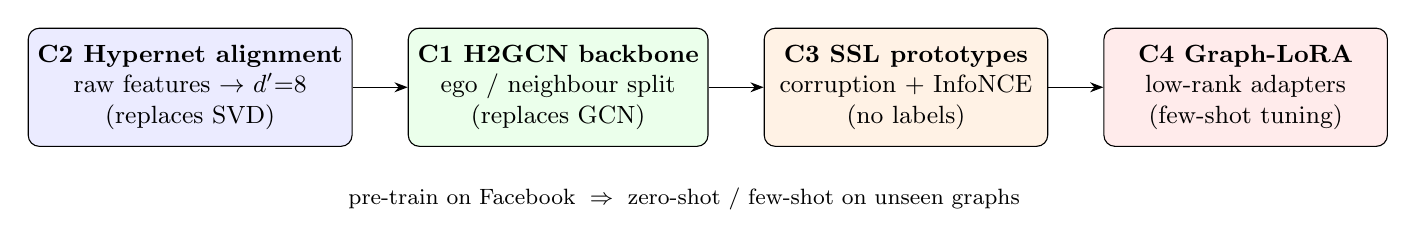
\begin{tikzpicture}[box/.style={draw,rounded corners,align=center,minimum width=3.6cm,minimum height=1.5cm,font=\small},>=Stealth]
\node[box,fill=blue!8] (a) {\textbf{C2 Hypernet alignment}\\raw features $\to$ $d'{=}8$\\(replaces SVD)};
\node[box,fill=green!8,right=0.7cm of a] (b) {\textbf{C1 H2GCN backbone}\\ego / neighbour split\\(replaces GCN)};
\node[box,fill=orange!10,right=0.7cm of b] (c) {\textbf{C3 SSL prototypes}\\corruption + InfoNCE\\(no labels)};
\node[box,fill=red!8,right=0.7cm of c] (d) {\textbf{C4 Graph-LoRA}\\low-rank adapters\\(few-shot tuning)};
\draw[->] (a)--(b); \draw[->] (b)--(c); \draw[->] (c)--(d);
\node[below=0.4cm of b,xshift=1.6cm,font=\footnotesize] {pre-train on Facebook $\;\Rightarrow\;$ zero-shot / few-shot on unseen graphs};
\end{tikzpicture}
\end{frame}

\begin{frame}{C1: H2GCN -- heterophily-aware backbone}
\begin{columns}[T]
\column{0.52\textwidth}
\textbf{Why:} GCN's self-loop averages a node into its neighbours, shrinking the residual the detector needs.\\[4pt]
\textbf{How (H2GCN principles):} ego/neighbour separation, 1- and 2-hop, combine:
\[
\text{out}=\sigma\big(XW_{e}+A_nXW_1+A_n^2XW_2+b\big),\; A_n=\hat A-I
\]
Drop-in for the paper's GCN; params $484$k$\to811$k.
\column{0.48\textwidth}
\small
\begin{tabular}{lccc}
\toprule
AUROC & Amazon & UPU & Reddit\\ \midrule
Baseline & \textbf{.834} & \textbf{.792} & .564\\
+C1 & \textcolor{bad}{.668} & \textcolor{bad}{.701} & .589\\ \bottomrule
\end{tabular}\\[4pt]
\begin{itemize}\footnotesize
\item Learns in-domain (FB-val .789 vs .828) but \alert{transfers worse}.
\item Reddit $+0.025$ is within noise.
\item Seed std 3$\times$ the baseline's.
\end{itemize}
\end{columns}
\end{frame}

\begin{frame}{C2: hypernetwork feature alignment}
\begin{columns}[T]
\column{0.52\textwidth}
\textbf{Why:} SVD is linear and fitted per graph; its components mean different things in different graphs.\\[4pt]
\textbf{How:} a hypernetwork generates a 2-layer non-linear projection from \emph{feature descriptors} (mean, skew, graph smoothness, \dots) and \emph{graph metadata} (size, density, \dots); works for any width $D$.
\[
W_1[j]=g_1([z_j;m]),\; W_2=g_2(m)
\]
23k extra parameters; trained end-to-end.
\column{0.48\textwidth}
\small
\begin{tabular}{lccc}
\toprule
AUROC & Amazon & UPU & Reddit\\ \midrule
Baseline & \textbf{.834} & \textbf{.792} & .564\\
+C2 & \textcolor{bad}{.418} & \textcolor{bad}{.398} & .584\\ \bottomrule
\end{tabular}\\[4pt]
\begin{itemize}\footnotesize
\item \alert{Below chance} on Amazon (ranking inverted).
\item In-domain it learns (.750).
\item Likely cause: one training graph $=$ one metadata point; nothing teaches how the projection should vary (\emph{untested}).
\end{itemize}
\end{columns}
\end{frame}

\begin{frame}{C3: contrastive prototype learning with \alert{no labels}}
\begin{columns}[T]
\column{0.52\textwidth}
\textbf{Why:} the paper needs labelled anomalies; they are scarce.\\[4pt]
\textbf{How:} corrupt the training graph each epoch (rewire 5\% of neighbourhoods, swap features of 5\% of node pairs) $\Rightarrow$ corrupted nodes = pseudo-abnormal.
\begin{itemize}\footnotesize
\item \textbf{Prototype InfoNCE:} residual must pick its pseudo-class prototype ($\tau{=}0.2$, class-balanced)
\item \textbf{View InfoNCE:} clean-view node retrieves itself in the corrupted view
\end{itemize}
\column{0.48\textwidth}
\small
\begin{tabular}{lccc}
\toprule
AUROC & Amazon & UPU & Reddit\\ \midrule
Supervised baseline & \textbf{.834} & \textbf{.792} & .564\\
\textbf{C3, no labels} & .620 & .588 & .585\\ \bottomrule
\end{tabular}\\[4pt]
\begin{itemize}\footnotesize
\item \textcolor{good}{\textbf{0.62 AUROC with zero labels}} (chance $=0.5$); in-domain .701.
\item Gap to supervision: random corruption $\ne$ camouflaged fraud.
\item Can use \emph{any} unlabelled graph $\to$ multi-source.
\end{itemize}
\end{columns}
\end{frame}

\begin{frame}{C4: Graph-LoRA for few-shot adaptation}
\begin{columns}[T]
\column{0.5\textwidth}
\textbf{How:} freeze the GNN; learn $W'=W+\tfrac{\alpha}{r}BA$ ($r{=}4$, $B{=}0$ at init); toggle on/off.\\[6pt]
\small
\begin{tabular}{lr}
\toprule
Method & Trainable params\\ \midrule
Prompt (paper idea) & 80\\
\textbf{Graph-LoRA} & \textbf{4,832}\\
Full GNN fine-tune & 164,002\\ \bottomrule
\end{tabular}\\[4pt]
\textcolor{good}{LoRA $=$ 2.9\% of full fine-tuning.}
\column{0.5\textwidth}
\footnotesize
\begin{tabular}{lccc}
\toprule
AUROC & Amazon & UPU & Reddit\\ \midrule
zero-shot baseline & .834 & .792 & .564\\
LoRA (paper budget) & .834 & .793 & .563\\
Full FT (paper budget) & .839 & .795 & .563\\
LoRA (30 ep, 1e-3)* & .651 & .693 & .608\\
Full FT (30 ep, 1e-3)* & .637 & .586 & .596\\
Prompt (30 ep, 1e-3)* & .851 & .797 & .568\\ \bottomrule
\end{tabular}\\[2pt]
\scriptsize *sensitivity check, examined after seeing results.
\end{columns}
\vspace{2pt}
\begin{alertblock}{Honest reading}\footnotesize Efficiency claim holds; accuracy does not improve. Released few-shot code leaves its prompt commented out of \texttt{forward} --- it does no real tuning.\end{alertblock}
\end{frame}

\section{Results}
\begin{frame}{Main results: single training graph (Facebook)}
\centering\small
\begin{tabular}{lrccc}
\toprule
Method & Params & Amazon & Amazon-UPU & Reddit\\ \midrule
\textbf{Baseline AnomalyGFM} & 484,402 & \textbf{.834}{\tiny$\pm.022$} & \textbf{.792}{\tiny$\pm.017$} & .564{\tiny$\pm.026$}\\
+ C1 H2GCN & 810,802 & .668{\tiny$\pm.060$} & .701{\tiny$\pm.051$} & .589{\tiny$\pm.044$}\\
+ C2 Hypernet & 507,514 & .418{\tiny$\pm.092$} & .398{\tiny$\pm.055$} & .584{\tiny$\pm.043$}\\
+ C3 SSL (\emph{no labels}) & 484,002 & .620{\tiny$\pm.082$} & .588{\tiny$\pm.056$} & .585{\tiny$\pm.010$}\\
C1+C2+C3 combined & 833,914 & .529{\tiny$\pm.105$} & .543{\tiny$\pm.030$} & .550{\tiny$\pm.016$}\\ \bottomrule
\end{tabular}
\vspace{6pt}
\begin{itemize}\small
\item AUROC, mean$\pm$std over 5 seeds. \textbf{No extension beats the baseline on Amazon.}
\item Reddit differences ($\le0.025$) are within one std.
\item Peak GPU memory: extensions add only 4--5\% (Amazon: 508 $\to$ 511--533 MB).
\end{itemize}
\end{frame}

\begin{frame}{Do the modules learn? In-domain vs. transfer}
\centering\small
\begin{tabular}{lcc}
\toprule
Variant & Held-out Facebook AUROC & Amazon AUROC\\ \midrule
Baseline & 0.828 & 0.834\\
C1 H2GCN & 0.789 & 0.668\\
C2 Hypernet & 0.750 & 0.418\\
C3 SSL (no labels) & 0.701 & 0.620\\ \bottomrule
\end{tabular}
\vspace{6pt}
\begin{itemize}
\item Every module \textbf{learns} (all $\gg0.5$ in-domain) $\Rightarrow$ not a coding bug.
\item The failure is \textbf{transfer} from a single 1,081-node training graph (about 25 anomalies).
\item Next: does \alert{multi-source} pre-training fix it?
\end{itemize}
\end{frame}

\begin{frame}{Multi-source pre-training (target domain held out; 3 seeds)}
\centering\small
\begin{tabular}{lccc}
\toprule
AUROC & Amazon & Amazon-UPU & Reddit\\ \midrule
1-source (Facebook) baseline & \textbf{.832} & \textbf{.785} & .572\\
4-source baseline & \textcolor{bad}{.611} & \textcolor{bad}{.612} & .591\\
4-source + C1 H2GCN & .548 & .548 & .590\\
4-source + C2 Hypernet & .620 & .617 & \textcolor{bad}{.467}\\
4-source + C3 SSL (\emph{no labels}) & .573 & .576 & \textcolor{good}{\textbf{.610}}\\
4-source C1+C2+C3 & .530 & .508 & .476\\ \bottomrule
\end{tabular}
\vspace{4pt}
\begin{itemize}\footnotesize
\item Pool: Facebook, Reddit, Amazon, YelpChi, T-Finance minus the target's domain; large graphs as BFS subgraphs ($\le$4,000 nodes).
\item \textbf{Naive pooling hurt the supervised baseline} on Amazon ($-0.22$) --- negative transfer; Reddit $+0.02$ (noise).
\end{itemize}
\end{frame}

\begin{frame}{Reading the multi-source result}
\begin{columns}[T]
\column{0.5\textwidth}
\textbf{What the data support}
\begin{itemize}\small
\item \textcolor{good}{C2's inversion disappears} with 4 metadata points ($0.36\to0.62$): supports ``one graph $=$ one metadata point''.
\item \textcolor{good}{C3} is the best method on Reddit (0.610, label-free) --- suggestive, 3 seeds.
\item Adaptation again: no-op at paper budget; LoRA/full hurt on Amazon ($\approx0.45$), LoRA most stable on Reddit ($\pm.007$).
\end{itemize}
\column{0.5\textwidth}
\textbf{What we cannot claim}
\begin{itemize}\small
\item C2 still only \emph{matches} the degraded baseline and gets worse on Reddit.
\item Why pooling hurts is \alert{untested}: differing anomaly semantics? BFS-subgraph statistics $\ne$ full graph? our own SVD for Yelp/T-Fin? equal source weights?
\item It is ``naive pooling \emph{with our sampling}'' that fails --- not multi-source pre-training in general.
\end{itemize}
\end{columns}
\end{frame}

\section{Wrap-up}
\begin{frame}{What we learned}
\begin{enumerate}
\item \textbf{The paper reproduces} (Amazon $\approx0.83$--$0.86$) and our harness is exact (sparse $=$ dense).
\item \textbf{Cheap fixes don't work:} no re-scoring or re-normalising beat the paper (Exp H/I).
\item \textbf{Prototype problem:} normal/abnormal prototypes are nearly collinear; the paper's normal score is inverted.
\item \textbf{C3 is the useful idea:} anomaly structure can be learned with \alert{zero labels}.
\item \textbf{C4 gives efficiency, not accuracy:} 4,832 params vs 164,002, same accuracy at the paper's budget.
\item \textbf{C1/C2 do not transfer} from one small training graph --- negative results; \textbf{multi-source pooling} removes C2's inversion but hurts the baseline.
\item \textbf{Released few-shot code is a no-op} (prompt commented out).
\end{enumerate}
\end{frame}

\begin{frame}{Limitations and next steps}
\begin{columns}[T]
\column{0.5\textwidth}
\textbf{Limitations}
\begin{itemize}\small
\item One training graph (paper protocol), 5 seeds, 3 targets
\item No re-tuning of the larger models; we avoided tuning on target graphs (leakage)
\item Explanations of \emph{why} are hypotheses unless marked tested
\end{itemize}
\column{0.5\textwidth}
\textbf{Next steps}
\begin{itemize}\small
\item Camouflage-aware corruptions for C3
\item Use the abnormal prototype / pseudo-anomalies in few-shot objective (C4)
\item Prototype-separation loss (fix collinearity)
\item LoRA rank sweep; hypernet with a learned feature-set encoder
\end{itemize}
\end{columns}
\vspace{6pt}
\begin{block}{Code \& reports}\small github.com/SumitKumar-17/AnomalyGFM (branch \texttt{team-contributions}): \texttt{WORK.md}, \texttt{reports/C1--C4}, \texttt{evaluate\_team\_contributions.py}\end{block}
\end{frame}

\end{document}
